\chapter{आकाश में चंद्रमा}\label{ch:g2:moon-in-the-sky}

कुछ शामों को छतों के ऊपर चाँदी की एक पतली-सी मुस्कान टँगी होती है; दो
हफ़्ते बाद वही एक गोल लालटेन बनकर बग़ीचे को फीके उजाले से भर देती है।
यह वही \omterm{def:g2:moon-in-the-sky:moon}{चंद्रमा} है --- आकाश में हमारा सबसे पास का पड़ोसी, और अकेली
दूसरी दुनिया जिस पर इंसान कभी चला है। अब ठीक से जान-पहचान कर लेनी
चाहिए।

\section{आकाश में हमारा पड़ोसी}

\begin{definition}[चंद्रमा]\label{def:g2:moon-in-the-sky:moon}
\emph{चंद्रमा}\index{चंद्रमा} सलेटी चट्टान की एक विशाल गेंद है जो
पृथ्वी के चारों ओर चलती है --- अंतरिक्ष में हमारा वफ़ादार साथी। वह
पृथ्वी से बहुत छोटा है, और बहुत दूर --- किसी भी हवाई जहाज़ की उड़ान
से कहीं दूर, इतनी दूर कि वहाँ जाने वाले अंतरिक्ष-यात्रियों को तीन दिन
सफ़र करना पड़ा।
\end{definition}

\begin{example}[ध्यान से देखने पर]\label{ex:g2:moon-in-the-sky:closely}
नंगी आँख से \omterm{def:g2:moon-in-the-sky:moon}{चंद्रमा} पर फीके धब्बे और चमकीले इलाक़े दिखते हैं ---
कुछ लोगों को उनमें कोई चेहरा नज़र आता है। दूरबीन से (\omterm{ex:g2:moon-in-the-sky:shapes}{पूर्ण चंद्र} वाली
रात इसे ज़रूर आज़माना) वे धब्बे साफ़ होकर मैदानों और गोल
\emph{क्रेटरों} में बदल जाते हैं, यानी कटोरे जैसे उन गड्ढों में जो
बहुत पहले अंतरिक्ष से आई चट्टानों के टकराने से बने। \omterm{def:g2:moon-in-the-sky:moon}{चंद्रमा} अपने ये
निशान हमेशा के लिए सँभाले रखता है: उन्हें मिटाने के लिए वहाँ न \omterm{def:g2:air-around-us:wind}{पवन} है
न बारिश --- सच तो यह है कि वहाँ \omterm{def:g2:air-around-us:air}{हवा} ही नहीं है। \omterm{def:g2:air-around-us:air}{हवा} न होने का एक
मतलब यह भी है कि वह दुनिया चुप है: \omterm{def:g2:moon-in-the-sky:moon}{चंद्रमा} पर चीख़ की भी कोई आवाज़
नहीं होती।
\end{example}

\begin{omfigure}
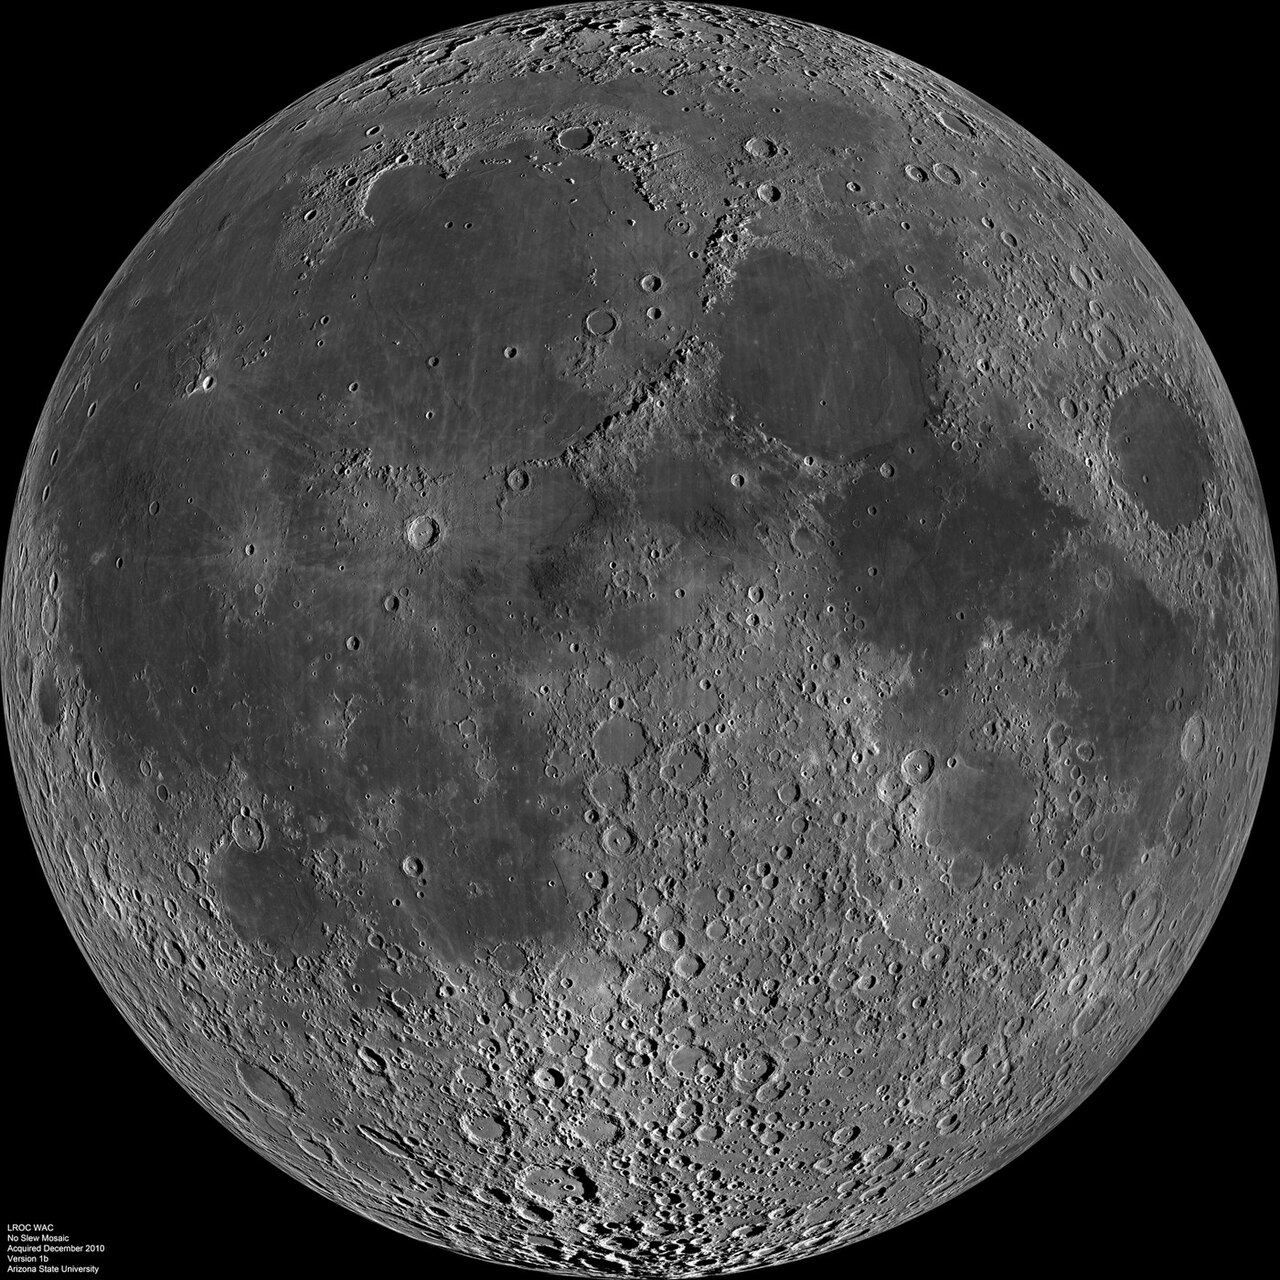
\includegraphics[width=0.44\linewidth]{images/book1/moon-nearside-lro.jpg}

{\small कक्षा से खींचा गया \omterm{def:g2:moon-in-the-sky:moon}{चंद्रमा} का चेहरा: चारों ओर कटोरे जैसे
क्रेटर, चौड़े गहरे मैदान --- और न \omterm{def:g2:air-around-us:air}{हवा}, न \omterm{def:g2:air-around-us:wind}{पवन}, न आवाज़।
\emph{चित्र: नासा/जीएसएफ़सी/एरिज़ोना स्टेट यूनिवर्सिटी।}}
\end{omfigure}

\begin{example}[पीछे-पीछे आता चंद्रमा]\label{ex:g2:moon-in-the-sky:follows}
चाँदनी शाम को सड़क पर चलो: घर और पेड़ पीछे सरकते जाते हैं, पर \omterm{def:g2:moon-in-the-sky:moon}{चंद्रमा}
मानो तुम्हारे पीछे-पीछे चलता है, हमेशा तुम्हारे कंधे के पास। वह
सचमुच तुम्हारा पीछा नहीं कर रहा --- वह इतना दूर है कि पूरी सड़क चल
लेने से भी उसका नज़ारा ज़रा नहीं बदलता, जबकि पास के घरों का नज़ारा हर
पल बदलता रहता है। बहुत दूर की चीज़ें हर राही के पीछे-पीछे चलती लगती
हैं; \omterm{def:g2:moon-in-the-sky:moon}{चंद्रमा} यह काम सबसे अच्छा करता है, क्योंकि दूरी में वही चैंपियन
है।
\end{example}

\section{परावर्तित प्रकाश}

\begin{example}[चाँदनी असल में सूर्य का प्रकाश है]\label{ex:g2:moon-in-the-sky:borrowed}
क्या \omterm{def:g2:moon-in-the-sky:moon}{चंद्रमा} \omterm{def:g1:light-and-shadows:source}{प्रकाश स्रोत} है? पिछले साल वाली जाँच याद करो: क्या वह
अपना \omterm{def:g1:light-and-shadows:source}{प्रकाश} ख़ुद बनाता है? नहीं --- \omterm{def:g2:moon-in-the-sky:moon}{चंद्रमा} तो गहरी चट्टान की गेंद
है, आकाश में रखे किसी विशाल कंकड़ जैसा। जिसे हम चाँदनी कहते हैं, वह
उसी चट्टान से \emph{परावर्तित} हुआ सूर्य का \omterm{def:g1:light-and-shadows:source}{प्रकाश} है --- हमारी ओर
लौटाया हुआ, ठीक वैसे जैसे सफ़ेद दीवार बिना लैंप बने कमरे को उजाला
देती है। सूर्य \omterm{def:g2:moon-in-the-sky:moon}{चंद्रमा} के एक हिस्से को चमकीला कर देता है; हमें उस
चमकीले हिस्से का उतना ही भाग दिखता है जितना हमारी ओर होता है।
\end{example}

\begin{omfigure}
\begin{tikzpicture}[scale=0.85]
  \fill[omThm] (0.7,1.5) circle (0.45);
  \foreach \a in {0,30,...,330} {
    \draw[omThm] (0.7,1.5) ++(\a:0.62) -- ++(\a:0.26);
  }
  \node[below, font=\small] at (0.7,0.8) {सूर्य};
  \draw[thick] (6.8,1.5) circle (1.1);
  \begin{scope}
    \clip (6.8,1.5) circle (1.1);
    \fill[omExo, opacity=0.5] (6.8,0.3) rectangle (8.1,2.7);
  \end{scope}
  \node[below, font=\small] at (6.8,0.1)
    {धूप वाला हिस्सा उजला, दूर वाला अँधेरा};
\end{tikzpicture}

{\small सूर्य \omterm{def:g2:moon-in-the-sky:moon}{चंद्रमा} के आधे हिस्से को उजाला देता है, और हमेशा उसी
आधे को जो उसके सामने हो। दूसरे आधे हिस्से में अपनी रात चल रही होती
है।}
\end{omfigure}

\begin{remark}[दिन का चंद्रमा]\label{rem:g2:moon-in-the-sky:daytime}
बहुत-से लोग मानते हैं कि \omterm{def:g2:moon-in-the-sky:moon}{चंद्रमा} रात का जीव है --- पर किसी दोपहर बाद
ऊपर देखो, और वह वहीं है, नीले आकाश में एक फीका-सा साया! \omterm{def:g2:moon-in-the-sky:moon}{चंद्रमा}
पृथ्वी के चारों ओर अपने ही समय पर चलता है और इसकी परवाह नहीं करता कि
हमारे यहाँ दिन है या रात। दिन में वह बस कम शान से दिखता है, जब सूर्य
की चौंध पूरे आकाश में भरी होती है।
\end{remark}

\section{चंद्रमा का आकार बदलता है}

\begin{example}[चंद्रमा के बदलते आकार]\label{ex:g2:moon-in-the-sky:shapes}
कई शामों तक \omterm{def:g2:moon-in-the-sky:moon}{चंद्रमा} को देखते रहो, तो उसका आकार बदलता है: पहले नाख़ून
की कतरन जैसा पतला \emph{बालचंद्र}\index{बालचंद्र}, फिर आधा गोला, फिर
मोटा-सा लगभग गोल आकार, और फिर \emph{पूर्ण चंद्र}\index{पूर्ण चंद्र}
की पूरी थाली --- और उसके बाद वापस घटते हुए, दूसरी ओर मुड़ा हुआ
\omterm{ex:g2:moon-in-the-sky:shapes}{बालचंद्र}, जब तक कि एक-दो रातों के लिए \omterm{def:g2:moon-in-the-sky:moon}{चंद्रमा} पूरी तरह ग़ायब न लगने
लगे। यह पूरा तमाशा लगभग एक महीने में होता है, और फिर दोहरा जाता है ---
दिन और रात जितने भरोसे के साथ।
\end{example}

\begin{omfigure}
\begin{tikzpicture}[scale=0.85]
  % dark disc for every station, lit part painted over it
  \foreach \x in {0,2.2,4.4,6.6,8.8} {
    \fill[omExo!75] (\x,0) circle (0.8);
  }
  % crescent: lit right edge only
  \begin{scope}
    \clip (2.2,0) circle (0.8);
    \fill[yellow!30] (2.2,-0.85) rectangle (3.05,0.85);
    \fill[omExo!75] (2.2,0) ellipse (0.5 and 0.8);
  \end{scope}
  % half: lit right half
  \begin{scope}
    \clip (4.4,0) circle (0.8);
    \fill[yellow!30] (4.4,-0.85) rectangle (5.25,0.85);
  \end{scope}
  % almost full: dark left sliver only
  \begin{scope}
    \clip (6.6,0) circle (0.8);
    \fill[yellow!30] (6.6,0) circle (0.8);
    \fill[omExo!75] (5.75,-0.85) rectangle (6.6,0.85);
    \fill[yellow!30] (6.6,0) ellipse (0.5 and 0.8);
  \end{scope}
  % full: all lit
  \fill[yellow!30] (8.8,0) circle (0.8);
  \foreach \x in {0,2.2,4.4,6.6,8.8} {
    \draw[thick] (\x,0) circle (0.8);
  }
  \node[below, font=\small] at (0,-1.05) {अमावस: छिपा हुआ};
  \node[below, font=\small] at (2.2,-1.05) {बालचंद्र};
  \node[below, font=\small] at (4.4,-1.05) {आधा};
  \node[below, font=\small] at (6.6,-1.05) {लगभग पूरा};
  \node[below, font=\small] at (8.8,-1.05) {पूर्ण चंद्र};
\end{tikzpicture}

{\small दो हफ़्ते \omterm{def:g2:moon-in-the-sky:moon}{चंद्रमा} को देखने पर: उजला आकार रात-दर-रात बढ़ता
जाता है, कुछ भी न होने से लेकर पूरी थाली तक --- और फिर घटने लगता है।}
\end{omfigure}

\begin{omfigure}
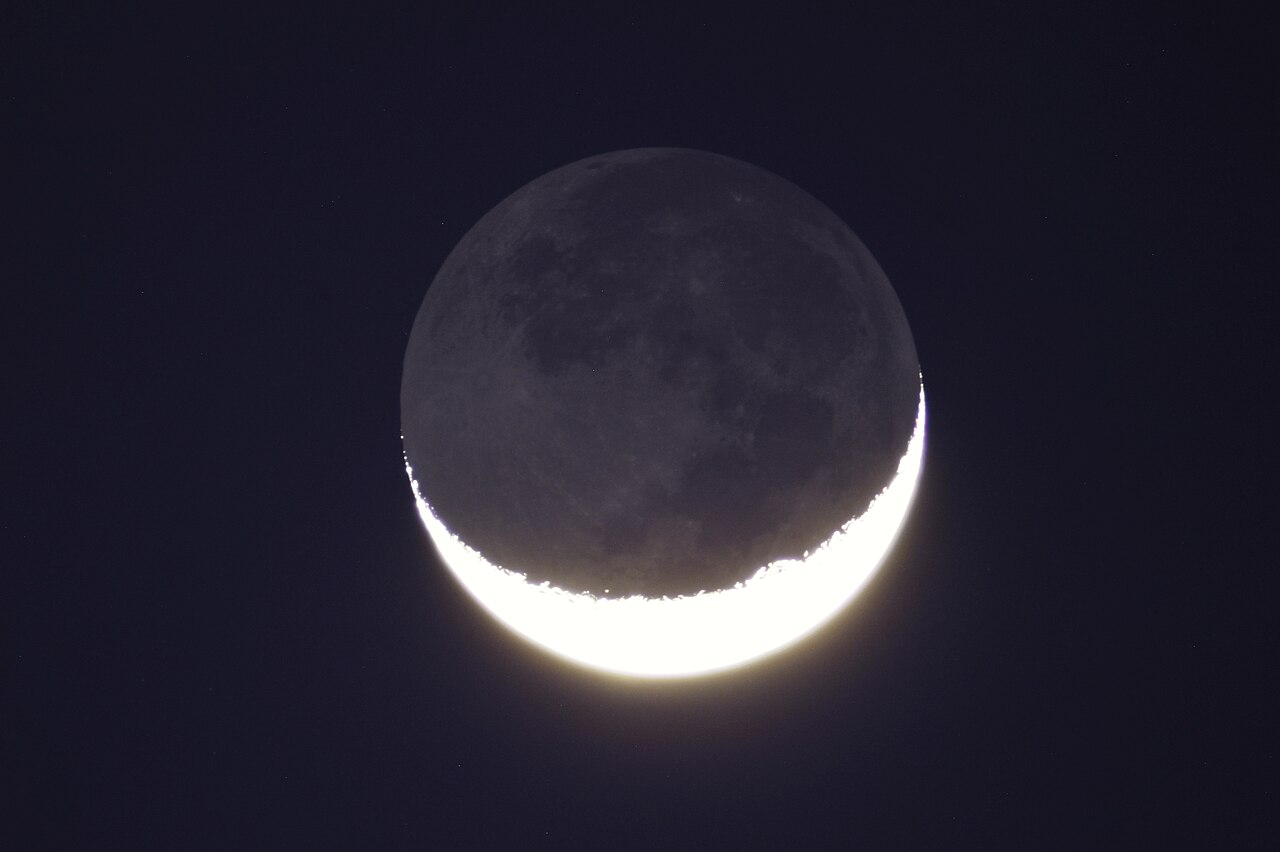
\includegraphics[width=0.42\linewidth]{images/book1/moon-crescent.jpg}\quad
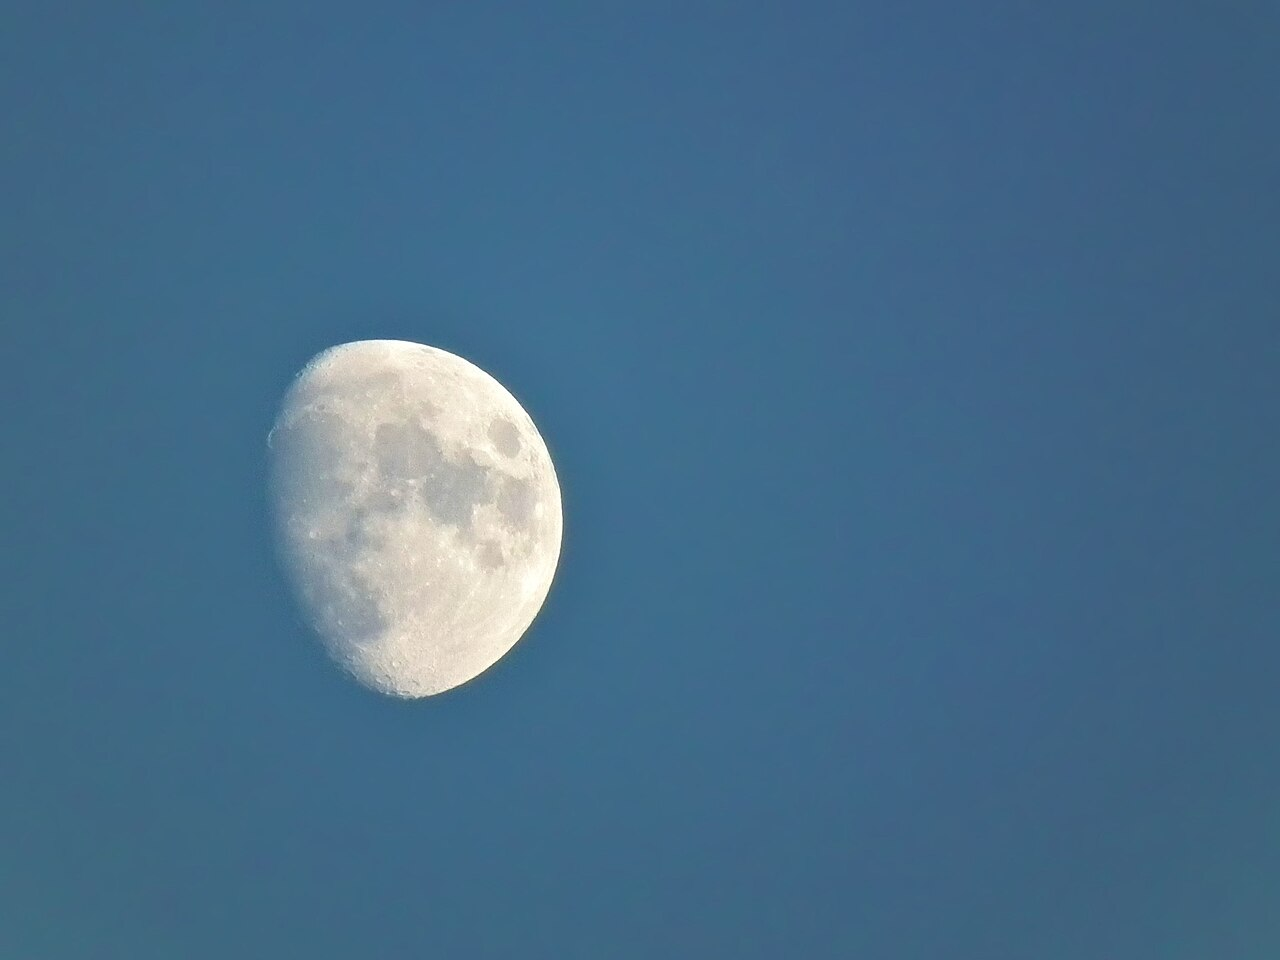
\includegraphics[width=0.42\linewidth]{images/book1/moon-gibbous.jpg}

{\small असली नज़ारा: एक पतला \omterm{ex:g2:moon-in-the-sky:shapes}{बालचंद्र} (बाएँ --- ध्यान से देखो: थाली
का अँधेरा हिस्सा भी हल्का-हल्का दमक रहा है) और दिन के आकाश में लगभग
पूरा \omterm{def:g2:moon-in-the-sky:moon}{चंद्रमा} (दाएँ)। \emph{चित्र: जी.~डोनातिएलो, CC0;
सीबाइल19, CC0.}}
\end{omfigure}

\begin{method}[चंद्रमा की डायरी रखना]\label{met:g2:moon-in-the-sky:diary}
\begin{enumerate}
  \item हर साफ़ शाम को, लगभग एक ही समय पर, \omterm{def:g2:moon-in-the-sky:moon}{चंद्रमा} को ढूँढ़ो;
  \item जो आकार दिखे उसे पंचांग के एक छोटे-से ख़ाने में बनाओ ---
        एक वृत्त, और अँधेरे हिस्से पर \omterm{def:g1:light-and-shadows:shadow}{छाया} कर दो;
  \item अगर बादल छिपा दें तो ``बादल'' लिख दो और आगे बढ़ जाओ;
  \item दो हफ़्ते बाद अपने सारे चित्र एक क़तार में रखो।
\end{enumerate}
तुम्हारे अपने चित्र दिखा देंगे कि आकार हर रात थोड़ा-थोड़ा बदलता है।
\omterm{def:g2:moon-in-the-sky:moon}{चंद्रमा} ऐसा \emph{क्यों} करता है, यह एक स्वादिष्ट पहेली है --- इसका
पूरा हल इस पाठ्यक्रम के किसी आगे वाले वर्ष में मिलेगा, और तुम्हारी
डायरी उस सबूत का पहला क़दम है।
\end{method}

\section{अभ्यास}

\begin{exercise}[$\star$]\label{exo:g2:moon-in-the-sky:1}
\omterm{def:g2:moon-in-the-sky:moon}{चंद्रमा} पृथ्वी से बड़ा है या छोटा? बादलों से पास है या दूर? हमें कैसे
पता कि लोग वहाँ जा सकते हैं?
\end{exercise}

\begin{exercise}[$\star$]\label{exo:g2:moon-in-the-sky:2}
\omterm{def:g2:moon-in-the-sky:moon}{चंद्रमा} पर कटोरे जैसे गोल निशानों को क्या कहते हैं, और वे बने किससे?
इतने समय बाद भी वे वहाँ क्यों हैं?
\end{exercise}

\begin{exercise}[$\star$]\label{exo:g2:moon-in-the-sky:3}
\omterm{def:g2:moon-in-the-sky:moon}{चंद्रमा} लैंप जैसा \omterm{def:g1:light-and-shadows:source}{प्रकाश स्रोत} है, या सफ़ेद दीवार जैसा \omterm{def:g1:light-and-shadows:source}{प्रकाश}
लौटाने वाला? चाँदनी असल में आती कहाँ से है?
\end{exercise}

\begin{exercise}[$\star$]\label{exo:g2:moon-in-the-sky:4}
सूर्य \omterm{def:g2:moon-in-the-sky:moon}{चंद्रमा} के किस आधे हिस्से को उजाला देता है: हमेशा उसे जो सूर्य
के सामने हो, हमेशा उसी एक हिस्से को, या हर बार किसी भी हिस्से को?
\end{exercise}

\begin{exercise}[$\star$]\label{exo:g2:moon-in-the-sky:5}
क्या \omterm{def:g2:moon-in-the-sky:moon}{चंद्रमा} दिन में भी दिख सकता है? अगर कोई साथी मना करे, तो उसे
क्या दिखाकर मनाओगे?
\end{exercise}

\begin{exercise}[$\star$]\label{exo:g2:moon-in-the-sky:6}
\omterm{def:g2:moon-in-the-sky:moon}{चंद्रमा} के आकारों को क्रम में गिनाओ, नाख़ून की कतरन जैसे पतले आकार से
शुरू करके गोल लालटेन तक। यह पूरा तमाशा दोहराने से पहले लगभग कितने
समय तक चलता है?
\end{exercise}

\begin{exercise}[$\star$]\label{exo:g2:moon-in-the-sky:7}
\omterm{def:g2:moon-in-the-sky:moon}{चंद्रमा} पर \omterm{def:g2:air-around-us:air}{हवा} नहीं है। वहाँ चीख़ का क्या होगा? और पतंग का?
\end{exercise}

\begin{exercise}[$\star$]\label{exo:g2:moon-in-the-sky:8}
\cref{met:g2:moon-in-the-sky:diary} वाली \omterm{def:g2:moon-in-the-sky:moon}{चंद्रमा} की डायरी आज रात से
शुरू करो। डायरी को निष्पक्ष बनाने के लिए हर शाम कौन-सी दो चीज़ें एक
जैसी रहनी चाहिए?
\end{exercise}

\begin{exercise}[$\star\star$]\label{exo:g2:moon-in-the-sky:9}
नन्ही रोज़ा कहती है, ``\omterm{def:g2:moon-in-the-sky:moon}{चंद्रमा} हमारी गाड़ी के पीछे-पीछे घर तक आया!''
\cref{ex:g2:moon-in-the-sky:follows} वाली सड़क की सैर से उसे समझाओ कि
बहुत दूर की चीज़ें पीछे-पीछे आती क्यों लगती हैं, जबकि पास की चीज़ें
सरककर पीछे रह जाती हैं।
\end{exercise}

\begin{exercise}[$\star\star$]\label{exo:g2:moon-in-the-sky:10}
\omterm{ex:g2:moon-in-the-sky:shapes}{बालचंद्र} वाली रात में ध्यान से देखो: कभी-कभी \omterm{def:g2:moon-in-the-sky:moon}{चंद्रमा} का
\emph{अँधेरा} हिस्सा भी बहुत हल्का-हल्का दमकता है, इतना कि पूरे गोले
का अंदाज़ा लगाया जा सके। उस हिस्से पर सूर्य का \omterm{def:g1:light-and-shadows:source}{प्रकाश} तो नहीं पड़ता
--- पर पास ही कोई और चीज़ चमक रही है। कौन-सी बड़ी, चमकीली, धूप से
जगमगाती गेंद \omterm{def:g2:moon-in-the-sky:moon}{चंद्रमा} के अँधेरे हिस्से को उजाला दे सकती है, ठीक वैसे
जैसे \omterm{def:g2:moon-in-the-sky:moon}{चंद्रमा} हमारी रातों को देता है? (सुराग़: तुम उसी पर खड़े हो।)
\end{exercise}
